\documentclass[runningheads]{llncs}

\usepackage[hmargin=2cm,vmargin=2cm]{geometry}
\usepackage{amsmath}
\usepackage{booktabs}
\usepackage[pdfborder=000]{hyperref}
\usepackage{algorithm}
\usepackage{algorithmic}
\usepackage{graphicx}

\graphicspath{{figures/}}

\newcommand*{\term}{\frac{\lambda}{2}\sum_{i, j}W_{ij}^2(W_{ij}-1)^2(W_{ij}+1)^2}

\begin{document}
\title{Two Approaches to Extract Logical Rules for Mushroom Edibility: Neural Networks and Genetic Algorithm}
\author{Yuanbo Han}

\authorrunning{Yuanbo Han}

\institute{Research School of Computer Science\\ Australian National University\\
\email{u6617017@anu.edu.au}}

\maketitle

\begin{abstract}
The mushroom problem I investigate here, is to identify mushrooms as edible or poisonous, given their 22 biological attributes. The first method is to construct BP neural networks to perform this task, preprocessed with data mining techniques. It avoids enumeration as a decision tree requires. The cost function is the conventional MSE (mean square error), plus a convergence controller. This additional term forces weights to approach 1, 0 or -1 under adequate training. Such being the case, the networks can be interpreted as a tree-like logical graph, in which $weight=1$ means positively related, $-1$ negatively, and $0$ irrelevant. As a result, the top 4 logical rules cover 100\% accuracy. The second method is a combination of Genetic Algorithm (GA) for feature selection and Decision Tree, where the accuracy of Decision Tree built by GA selected features serves back as the GA fitness function.

\keywords{Rule Extraction \and Mushroom Classification\and Neural Networks \and Genetic Algorithm \and Decision Tree.}
\end{abstract}

\section{Introduction}
\label{sec-intro}
The mushroom dataset~\cite{lincoff1989audubon} includes descriptions of hypothetical samples corresponding to 23 species of gilled mushrooms in the Agaricus and Lepiota Family (pp. 500-525). Each species is identified as definitely edible, definitely poisonous, or of unknown edibility and not recommended. The latter class was combined with the poisonous one. By convention, people always hope to grasp some rules for classifying edibility with the naked eye. Nevertheless, there is no simple rule for determining the edibility of a mushroom; no rule like ``leaflets three, let it be'' for Poisonous Oak and Ivy. So my target is trying to extract, if any, some easy rules with high application value. With these possible rules, people could instantly make a reliable judgment.

Admittedly, we have a theoretically deterministic method to obtain all the logical rules for this kind of problem---Decision Tree. However, this extraction approach has an exponential complexity. A decision tree with 22 attributes is seriously intractable. My solution is to make full use of logically interpretable neural networks, so that prune those features of little concern. In the ideal case, not many attributes are left to be considered, and we might easily see the connections between those principal features and edibility class.

One thing worth mentioning is that, edibility as a binary attribute (edible or poisonous) is asymmetric. In other words, false negative (wrongly identified as poisonous) is generally acceptable, but false positive (incorrectly identified as edible) can be fatal! So when encountering a trade-off, we would rather sacrifice the overall accuracy than miss only one poisonous sample.

The original data contains 8124 instances, with 22 attributes and 1 class (all nominally valued). To implement a neural networks classifier, I first quantize the values by a data mining technique. And then construct a single-hidden-layer BP neural network. For such a binary classification problem, only one output neuron is needed. Based on the traditional MSE, an auxiliary term is added to the cost function~\cite{duch1996extraction}. Mathematically, it is $\term$, where $W$ is the weight between input and hidden layer. 

After training, formalize the weights to be their nearest integer (i.e. 1, 0 or -1). $W$ is actually a sparse matrix, which suggests that many attribute values are irrelevant to the mushroom's edibility. Under the circumstances, enumerating all the related variables and combining them works out well.

\section{Data Preprocessing}
There are a range of measures to quantize a nominal value within Data Mining's scope (take a shot at Table~\ref{attr} below). Here, the vast majority of attributes have no concept for comparison. That is, you can not say brown cap-color is better/larger/longer than red cap-color. So I choose to apply a dimensional discretization. For each attribute, fix a sequence of al the unique values, and then build a Euclidean space with dimension = number of unique values. The quantized value is such a vector that all of the coordinates equal to $-1$, except the corresponding position being $1$. For the missing value, just regard it as another unique meaningful value.

Take cap-shape feature as an example.

\qquad All the unique nominal values are:

\qquad\qquad bell=b, conical=c, convex=x, flat=f, knobbed=k, sunken=s

\qquad There are 6 unique values. Fix this order, and perform discretization as described above.

\qquad Then b becomes $(1, -1, -1, -1, -1, -1)$, x becomes $(-1, -1, 1, -1, -1, -1)$, etc.

As for the class (edibility), I encode 1 for edible and 0 for poisonous.

Finally, each instance is a 126-dimension vector (125 variables and 1 class). They will be passed respectively as inputs and the target in the neural networks. After doing discretization, randomly select 20\% of the instances as the test set, and the rest being training set.

\begin{table}
\caption{Mushroom Attributes}
\label{attr}
\centering
\begin{tabular}{ll}
	\toprule
	Attribute & Values \\
	\midrule
	1. cap-shape & bell=b,conical=c,convex=x,flat=f,knobbed=k,sunken=s \\
	2. cap-surface & fibrous=f,grooves=g,scaly=y,smooth=s \\
	3. cap-color & brown=n,buff=b,cinnamon=c,gray=g,green=r,\\
	& pink=p,purple=u,red=e,white=w,yellow=y \\
	4. bruises? & bruises=t,no=f \\
	5. odor & almond=a,anise=l,creosote=c,fishy=y,foul=f,musty=m,none=n,pungent=p,spicy=s \\
	6. gill-attachment & attached=a,descending=d,free=f,notched=n \\
	7. gill-spacing & close=c,crowded=w,distant=d \\
	8. gill-size & broad=b,narrow=n \\
	9. gill-color & black=k,brown=n,buff=b,chocolate=h,gray=g,green=r,\\
	& orange=o,pink=p,purple=u,red=e,white=w,yellow=y \\
	10. stalk-shape & enlarging=e,tapering=t \\
	11. stalk-root & bulbous=b,club=c,cup=u,equal=e,rhizomorphs=z,rooted=r,missing=? \\
	12. stalk-surface-above-ring & fibrous=f,scaly=y,silky=k,smooth=s \\
	13. stalk-surface-below-ring & fibrous=f,scaly=y,silky=k,smooth=s \\
	14. stalk-color-above-ring & brown=n,buff=b,cinnamon=c,gray=g,orange=o,pink=p,red=e,white=w,yellow=y \\
	15. stalk-color-below-ring & brown=n,buff=b,cinnamon=c,gray=g,orange=o,pink=p,red=e,white=w,yellow=y \\
	16. veil-type & partial=p,universal=u \\
	17. veil-color & brown=n,orange=o,white=w,yellow=y \\
	18. ring-number & none=n,one=o,two=t \\
	19. ring-type & cobwebby=c,evanescent=e,flaring=f,large=l,none=n,pendant=p,sheathing=s,zone=z \\
	20. spore-print-color & black=k,brown=n,buff=b,chocolate=h,green=r,orange=o,purple=u,white=w,yellow=y \\
	21. population & abundant=a,clustered=c,numerous=n,scattered=s,several=v,solitary=y \\
	22. habitat & grasses=g,leaves=l,meadows=m,paths=p,urban=u,waste=w,woods=d \\
	\bottomrule
\end{tabular}
\end{table}

\section{BP Neural Networks}
\label{sec-bp}
As discussed above, my neural networks have a structure of one input layer of 125 variables (each equals to 1 or -1), one hidden layer with undefined units and exactly one output neuron. A diagrammatic sketch is shown in Figure~\ref{fig-bp}. The cost function is
\begin{equation}
	E(W) = MSE(Output, Target) + \term
\end{equation}
where $W_{ij}$ is the weight connecting $Input(i)$ and $Hidden(j)$.

When $W_{ij} = 1$, $-1$ or $0$, the second term derives its minimal (0), and the cost function turn back to MSE. This property promotes all the weights to approach one of $\{1, -1, 0\}$ during the training process with a proper $\lambda$. Meanwhile, freeze the weights between hidden and output layer as 1 (to reinforce the relationship).

\begin{figure}[htbp]
	\centering
	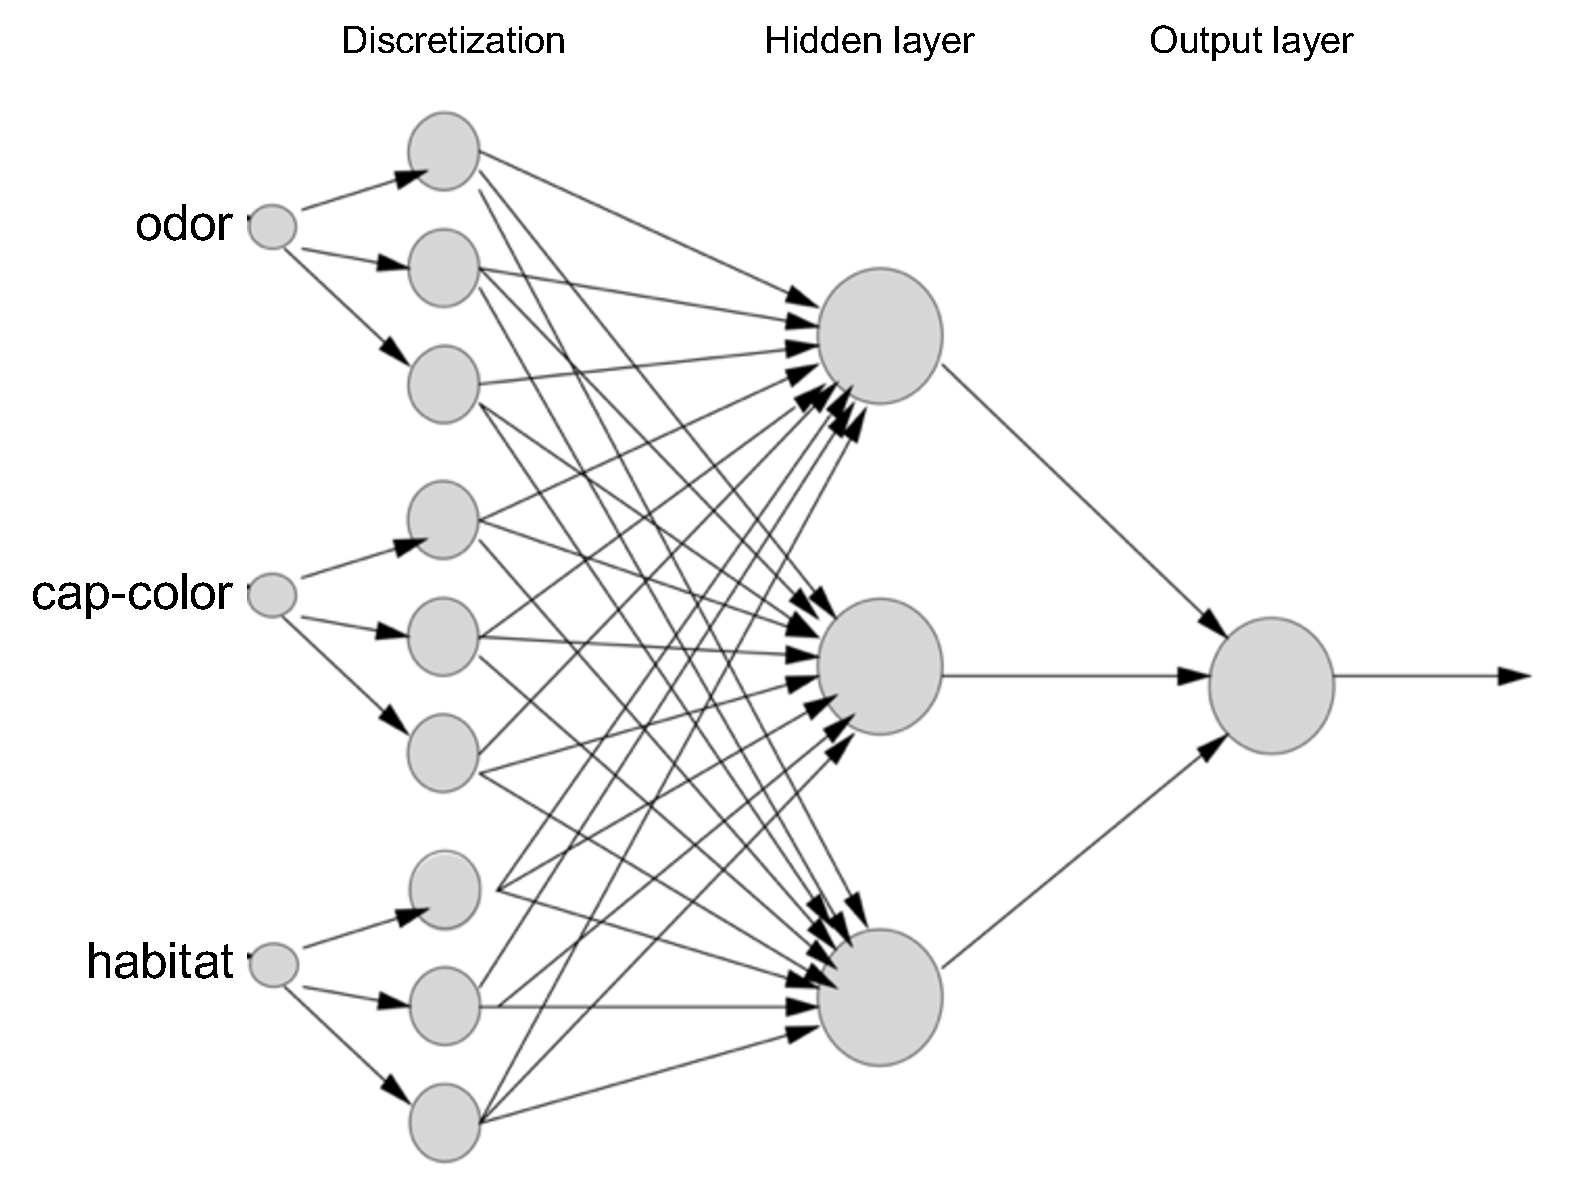
\includegraphics[scale=0.5]{bpNN}
	\caption{Sketch map of the BP neural networks}
	\label{fig-bp}
\end{figure}

Since the binary class has been encoded as 1 and 0, an appropriate choice of activation function for the output layer will be Sigmoid function ($\sigma(x) = \frac{1}{1+e^{-x}}$). Using this activation, the output lies in $(0,1)$. The classifier simply need to set a threshold (usually near 0.5), and compare the output with it. If $output > threshold$, then classify as 1 (edible); otherwise, poisonous.

Here, I would like to discuss why I set the cost function based on MSE rather than Cross-entropy. In the vast majority of cases, Softmax (which is the same as Sigmoid on binary classification) should be paired up with Cross-entropy. A number of papers can be found that analyze why they collaborate with each other. On the contrary, using Sigmoid with MSE is often a bad idea, because the derivatives are too small to change the weights when the output value is close to 0 or 1 due to Sigmoid function's flat slope. However, we never require the output value to approach as close to 0 or 1 as possible. Our ideal model is one that can accurately classify instances, and meanwhile the weights are near 1, 0 or -1. Figuratively speaking, it suffices to get an output of 0.2 or 0.75, no need rigidly demanding a value of 0.05 or 0.99. In the circumstances, it does not matter to use Sigmoid with MSE, for Sigmoid function is steep enough around 0.5. Furthermore, when it comes to the information of weights, MSE reflects better than Cross-entropy. This is true but kind of vague, so I do not strictly prove it here. To grasp an idea, imagine significantly changing the value of one weight, in all probability the cost function of MSE changes more than that of Cross-entropy. As a whole, MSE is sufficient for classification, and on the other hand performs outstandingly to adjust weights.

A trick part of this network is that the number of hidden units can not be too large. In fact, it should be really small such as 1--5. This is because our final target is to interpret the neural networks as logical rules. If there are many hidden neurons involved, the implicitly of topology can be really confusing.

For parameter adjustment, I have tried 1--3 hidden units, with changing the activation of hidden layer as Tanh function, Sigmoid function, etc. At the meantime, finetune $\lambda$ from 0.001 to 1. Also, fix the learning rate when needed. A strategy is to change $\lambda$ dynamically. At the preliminary stage of training, our main target is to make correct classifications, $\lambda$ should be small in case it influences the correct classification. With training carrying on, the accuracy will gradually reach a plateau, then the primary goal becomes forcing the weights to converge at an integer (1, 0 or -1), and $\lambda$ will matter during this phase. Through all kinds of attempts, the best setting of parameters can stably lead to 100\% accuracy on the training set itself.

Then I apply the model to the test set. The outcome with the same (best) parameters' setting is still 100\% accuracy. The data set is big enough (8124 instances), so the cross validation is unnecessary. Therefore, the result is to some extent reliable.

The Training Process is shown below. Note that we have to force the weights to be integers after training, so the Loss at last suddenly increases a little bit.
\begin{verbatim}
Epoch [1/3000] Loss: 0.2622  Accuracy: 50.640079 %
Epoch [201/3000] Loss: 0.0076  Accuracy: 99.766125 %
Epoch [401/3000] Loss: 0.0051  Accuracy: 99.876908 %
Epoch [601/3000] Loss: 0.0038  Accuracy: 99.901526 %
Epoch [801/3000] Loss: 0.0032  Accuracy: 99.987691 %
Epoch [1001/3000] Loss: 0.0028  Accuracy: 100.000000 %
Epoch [1201/3000] Loss: 0.0026  Accuracy: 100.000000 %
Epoch [1401/3000] Loss: 0.0025  Accuracy: 100.000000 %
Epoch [1601/3000] Loss: 0.0024  Accuracy: 100.000000 %
Epoch [1801/3000] Loss: 0.0023  Accuracy: 100.000000 %
Epoch [2001/3000] Loss: 0.0022  Accuracy: 100.000000 %
Epoch [2201/3000] Loss: 0.0021  Accuracy: 100.000000 %
Epoch [2401/3000] Loss: 0.0021  Accuracy: 100.000000 %
Epoch [2601/3000] Loss: 0.0020  Accuracy: 100.000000 %
Epoch [2801/3000] Loss: 0.0019  Accuracy: 100.000000 %
Epoch [3000/3000] Loss: 0.0139  Accuracy: 100.000000 %
\end{verbatim}

And the principal (mainly related) attributes are:
\begin{verbatim}
odor: [ 1  1 -1  0 -1  0  1 -1  0]
gill-spacing: [-1  1  0]
gill-size: [ 1 -1]
gill-color: [ 0  0 -1  0  0  0  0  0  0  0  0  0]
stalk-root: [-1  0  0  0  0  0  0]
stalk-surface-above-ring: [ 0  0 -1  0]
stalk-surface-below-ring: [ 0 -1  0  0]
stalk-color-below-ring: [1 0 0 0 0 0 0 0 0]
ring-type: [0 0 1 0 0 0 0 0]
spore-print-color: [ 1  1  0  0 -1  0  1  0  0]
population: [ 0 -1  0  0  0  1]
\end{verbatim}

As predicted before the experiment, only several variables contribute much to edibility. And now, using a Decision Tree method becomes practicable. Totally we get 12 distinct rules. Nonetheless, only the top 4 rules with most coverage can arrive an accuracy of 100\%.
\\\\
\begin{tabular}{c@{\qquad}l}
	Rule 1 & odor = NOT(almond OR anise OR none) \\
	& 120 cases missed, 98.52\% accuracy \\
	+ & \\
	Rule 2 & spore-print-color = green \\
	& 48 cases missed, 99.41\% accuracy \\
	+ & \\
	Rule 3 & odor = none AND stalk-surface-below-ring = scaly AND
	stalk-color-above-ring = NOT brown \\
	& 8 cases missed, 99.90\% accuracy \\
	+ & \\
	Rule 4 & habitat = leaves AND cap-color = white \\
	& 100\% accuracy \\
\end{tabular}
\\\\
A comparison is that \cite{schlimmer1987concept} gave a 95\% classification method in 1987.

\section{Improvements of BP Neural Networks}
Luckily, we succeed to derive easy rules for classification. However, situation exists when there is actually no easy, say involving at most 3 attributes, logical rules. Then we will get still complex variables after pruning by neural networks as discussed above. In this case, we may add another constraint term to the cost function, making it:
\begin{equation}
E(W) = MSE(Output, Target) + \term + \frac{\mu}{2}\sum_{ij}W_{ij}^2
\end{equation}

Similar to the second term, the new term acts like a attenuator, which guides those sub-important weights to be zero. Thus, we could again get few features after training. However, rules derived from this network are not highly reliable, because we have excluded too many factors including important but not dominating ones.

\section{GA + Decision Tree}
Briefly speaking, in this experiment, the objective is to extract simple crisp logical rules for mushroom edibility, and the main challenge is there are too many features. It is not easy to determine which feature to use. Traditionally, BP networks are good at classification, and adding an auxiliary term of weights to the cost function can guide the weights to converge to certain values. From the Bayesian point of view, such an auxiliary term actually changes the prior distribution of weights, making the density of 1, -1, 0 larger. Section~\ref{sec-bp} subtly solve the problem by this idea. However, the flaw is that one can not really interpret this new term. In other words, it has no real meaning, but only serves as a converging controller; and it works well just owing to persistently adjusting parameters. With other parameter settings, the network model can have a terribly poor performance.

The most intuitive approach for logical extraction is Decision Tree. But as Section~\ref{sec-intro} discussed, generally we could not simply apply a Decision Tree for this classification task, due to the excessive attributes and complexity of interpreting large trees. Then I come up with an approach---using Genetic Algorithm (GA) for feature selection. With only a few features selected by GA, constructing a Decision Tree becomes much easier.

Specifically, the structure of DNA is a 22-dimension binary array, since there are 22 features in total (see Table~\ref{attr}). Positive value (1) means the corresponding feature is in use, 0 the contrary. In addition to the normal GA, we fix a maximum number of positive features, called DNA\_POSITIVE. All the control parameters for GA are listed below:

\begin{table}
	\caption{GA Control Parameters}
	\label{tab-GA}
	\centering
	\begin{tabular}{l@{\qquad\qquad}l}
		\toprule
		Parameter & Meaning \\
		\midrule
		DNA\_SIZE = 22 & number of bits in DNA \\
		POP\_SIZE & population size \\
		DNA\_POSITIVE & max number of positive genes \\
		CROSS\_RATE & DNA crossover probability \\
		MUTATION\_RATE & mutation probability \\
		N\_GENERATIONS & generation size \\
		depth & max depth of Decision Tree \\
		\bottomrule
	\end{tabular}
\end{table}

In practice, a good setting is:
\begin{center}
	\begin{tabular}{l@{\quad=\quad}l}
		POP\_SIZE & 50 \\
		DNA\_POSITIVE & 3, 4, 5 \\
		CROSS\_RATE & 0.8 \\
		MUTATION\_RATE & 0.05 \\
		N\_GENERATIONS & 10 \\
		depth & 6 \\
	\end{tabular}
\end{center}

Having set related parameters, perform Algorithm~\ref{GA}. This is a combination of GA Feature Selection and Decision Tree, where the accuracy of Decision Tree built by GA selected features serves back as the GA fitness function. Note that line~11 shows a distinctive step---Depressing. After crossover and mutation, the offspring may well have more than DNA\_POSITIVE positive genes, so we randomly depress some of them (let them be 0 by force) till only DNA\_POSITIVE genes have value 1. Without such depressing procedure, the number of selected features would become lager and larger, leading to complicated trees again. More details are not necessary to discuss here, such as exception handling by initialization when there is no positive value (1) in a DNA, terminating in advance when accuracy reaches 100\%, etc.

\begin{algorithm}[htbp]
	\caption{GA Feature Selection + Decision Tree}
	\label{GA}
	\begin{algorithmic}
		\STATE Initialise population DNA
		\FOR {$g = 1 \sim \textrm{N\_GENERATIONS}$}
		\FOR {$p = 1 \sim \textrm{POP\_SIZE}$}
		\STATE Convert binary DNA to selected feature numbers
		\STATE Build a Decision Tree by selected features
		\STATE Report Decision Tree accuracy as the fitness function
		\ENDFOR
		\STATE Parent selection (Proportional strategy)
		\STATE Sexual uniform crossover
		\STATE Random mutation
		\STATE Depress redundant positive genes
		\STATE Replace parent immediately (Steady state GA)
		\ENDFOR
		\STATE Return the best DNA
	\end{algorithmic} 
\end{algorithm}

As a consequence,  the greatest accuracy is 99.7046\% on the whole data set (training + test) with DNA\_POSITIVE = 3. There is more than one choice of feature selection to obtain this biggest accuracy. An example is showed in Figure~\ref{fig-3}. With at least 4 features, the accuracy rate can reach 100\%. Nevertheless, introducing the 5th feature can simplify the Decision Tree topology compared with that of 4 features (see Figure~\ref{fig-4} and Figure~\ref{fig-5}). To interpret the encodings in Decision Tree graphs, please use the corresponding ``Feature List'' printed in Appendix, yet the interpreted rules are similar to those in Section~\ref{sec-bp}.

\begin{figure}[htbp]
	\centering
	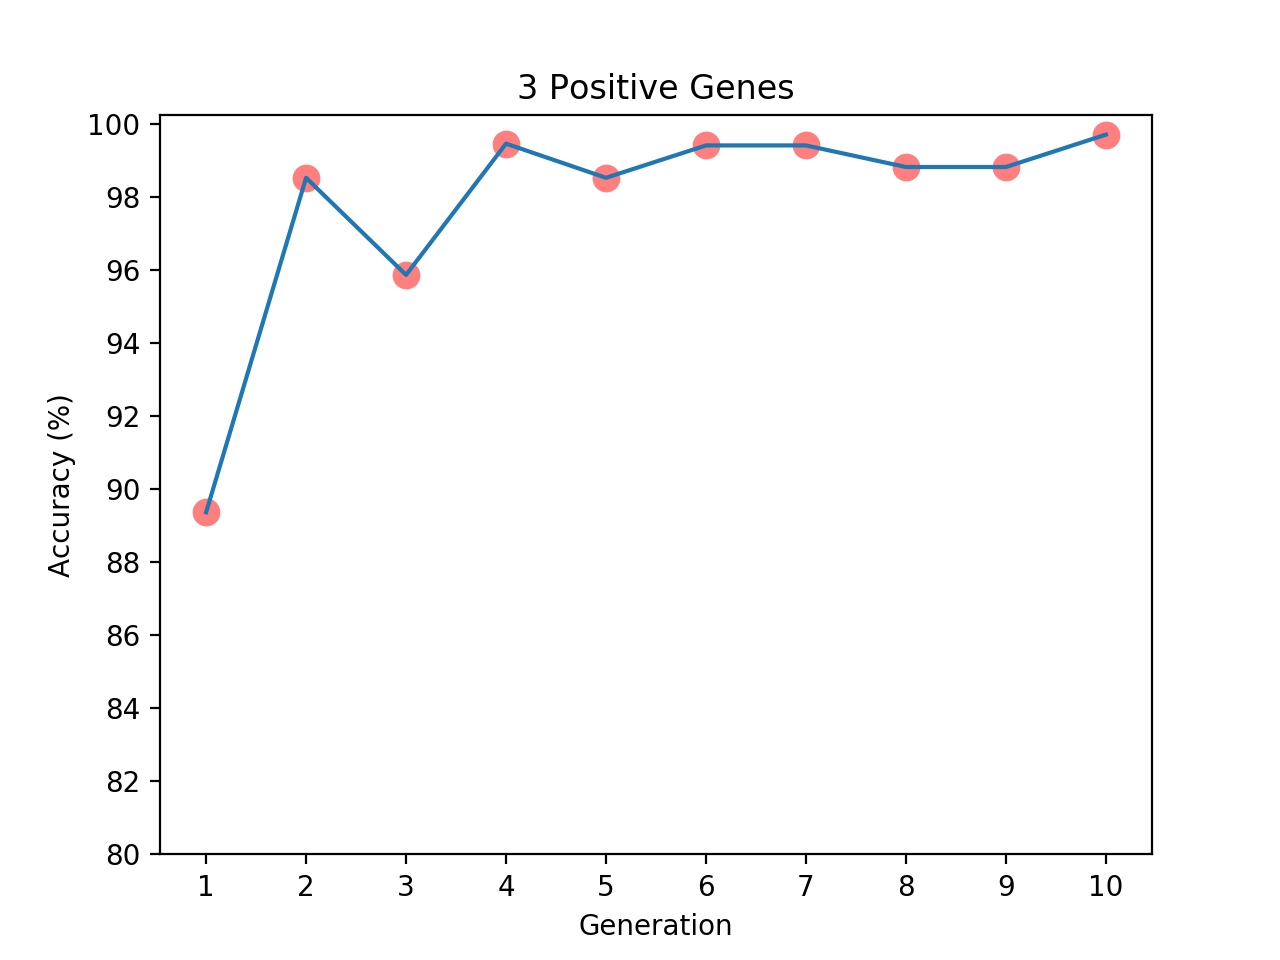
\includegraphics[scale=0.5]{GA3}
	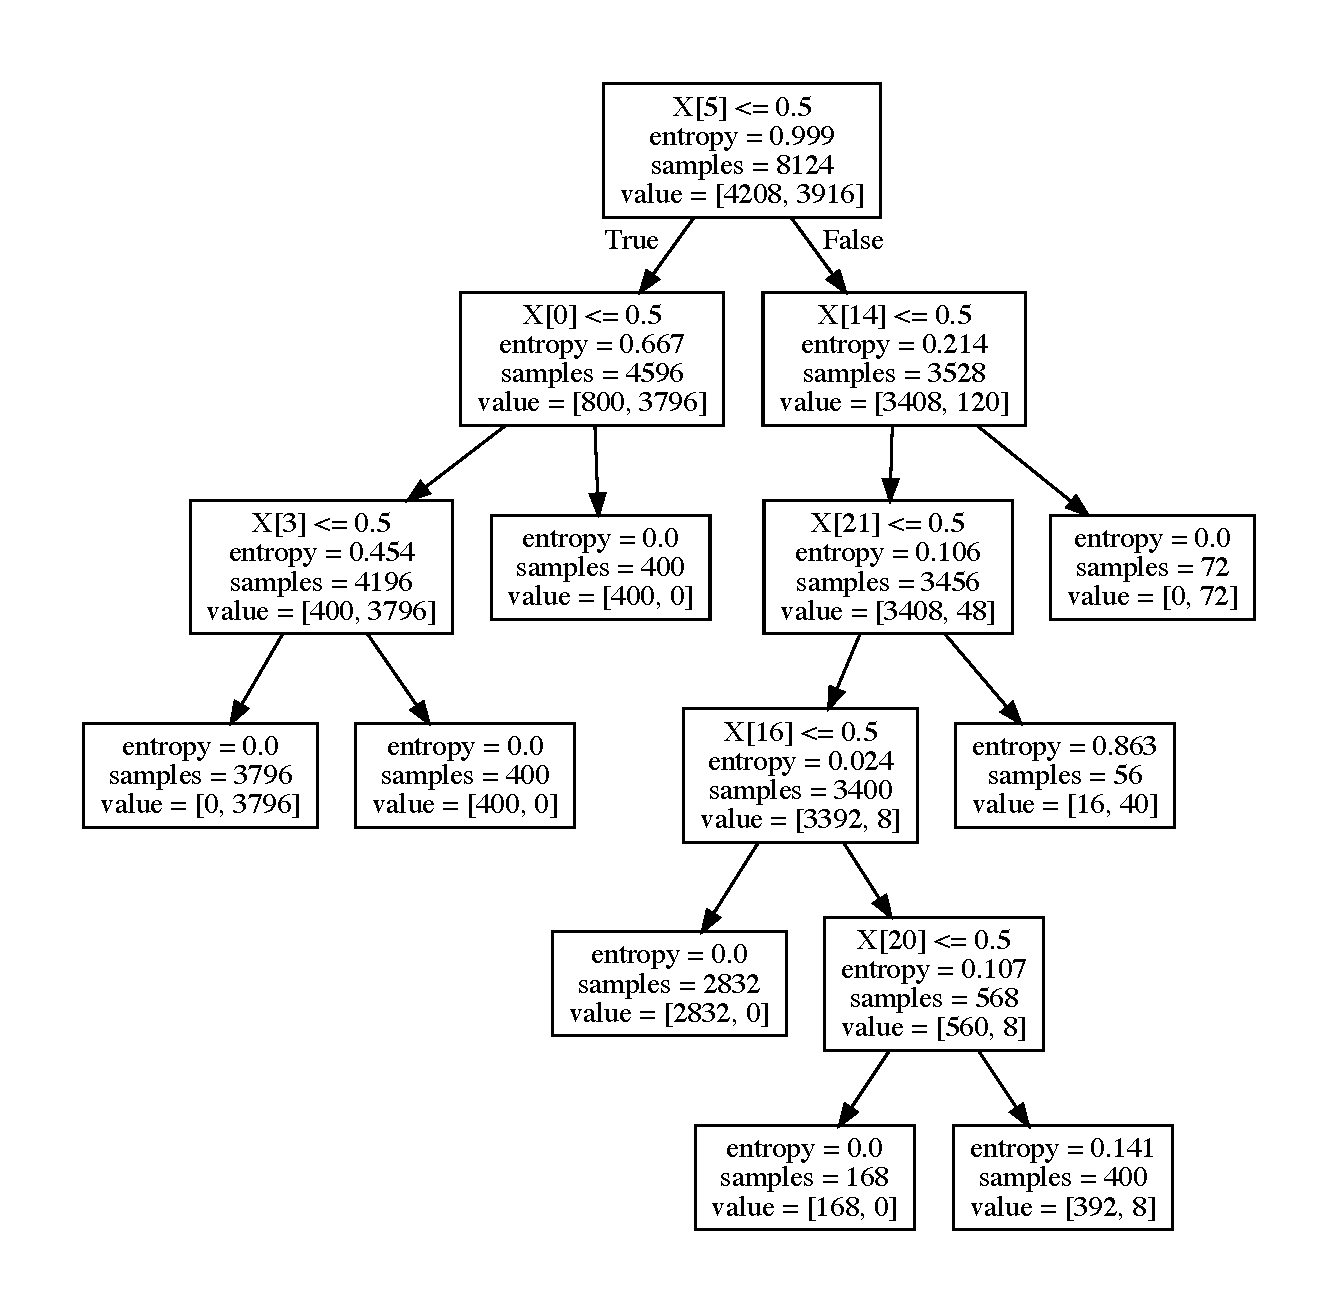
\includegraphics[scale=0.5]{tree3}
	\caption{GA process \& Decision Tree for 3 features}
	\label{fig-3}
\end{figure}

\begin{figure}[htbp]
	\centering
	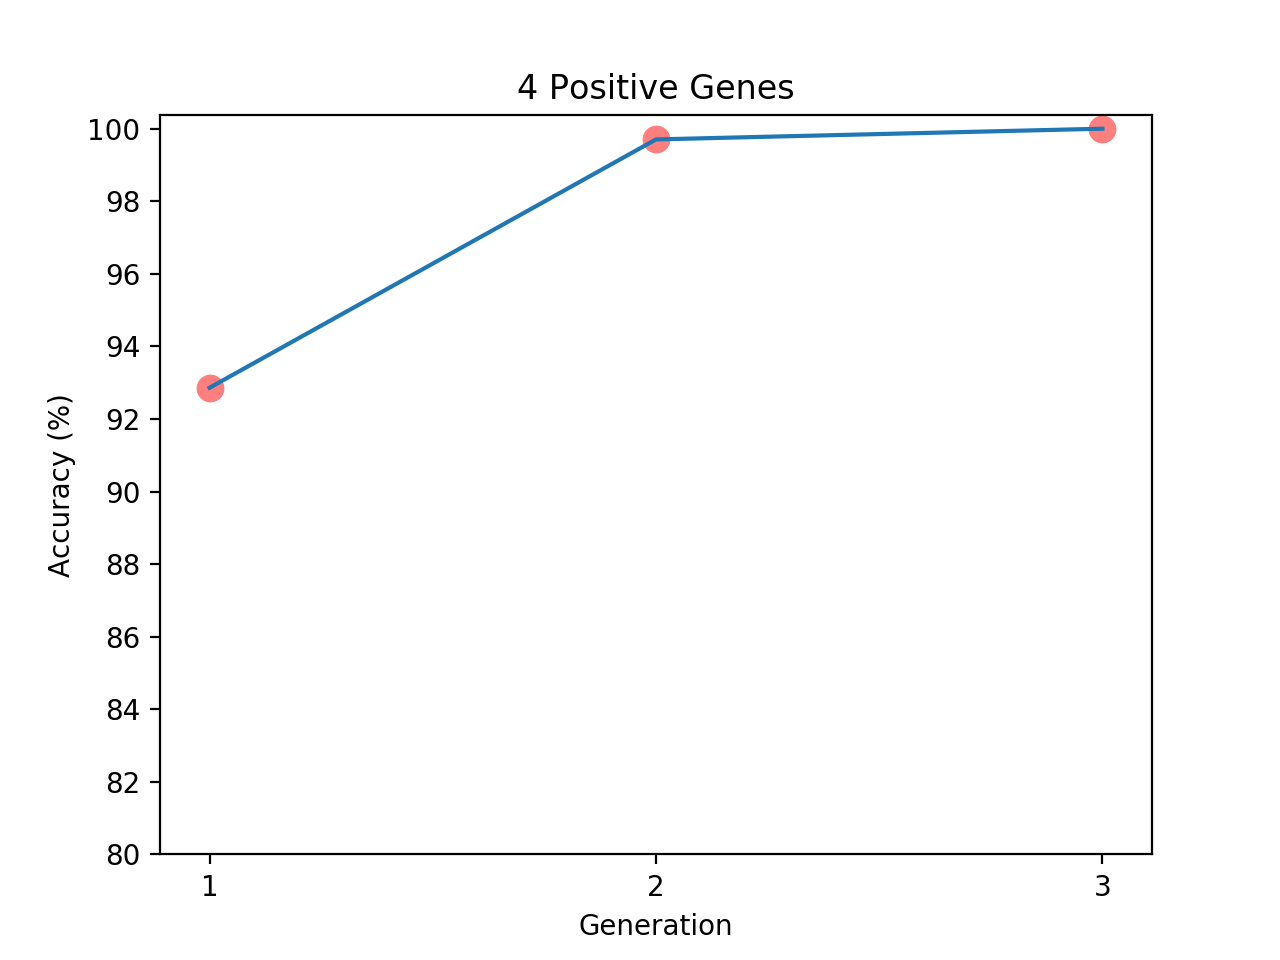
\includegraphics[scale=0.5]{GA4}
	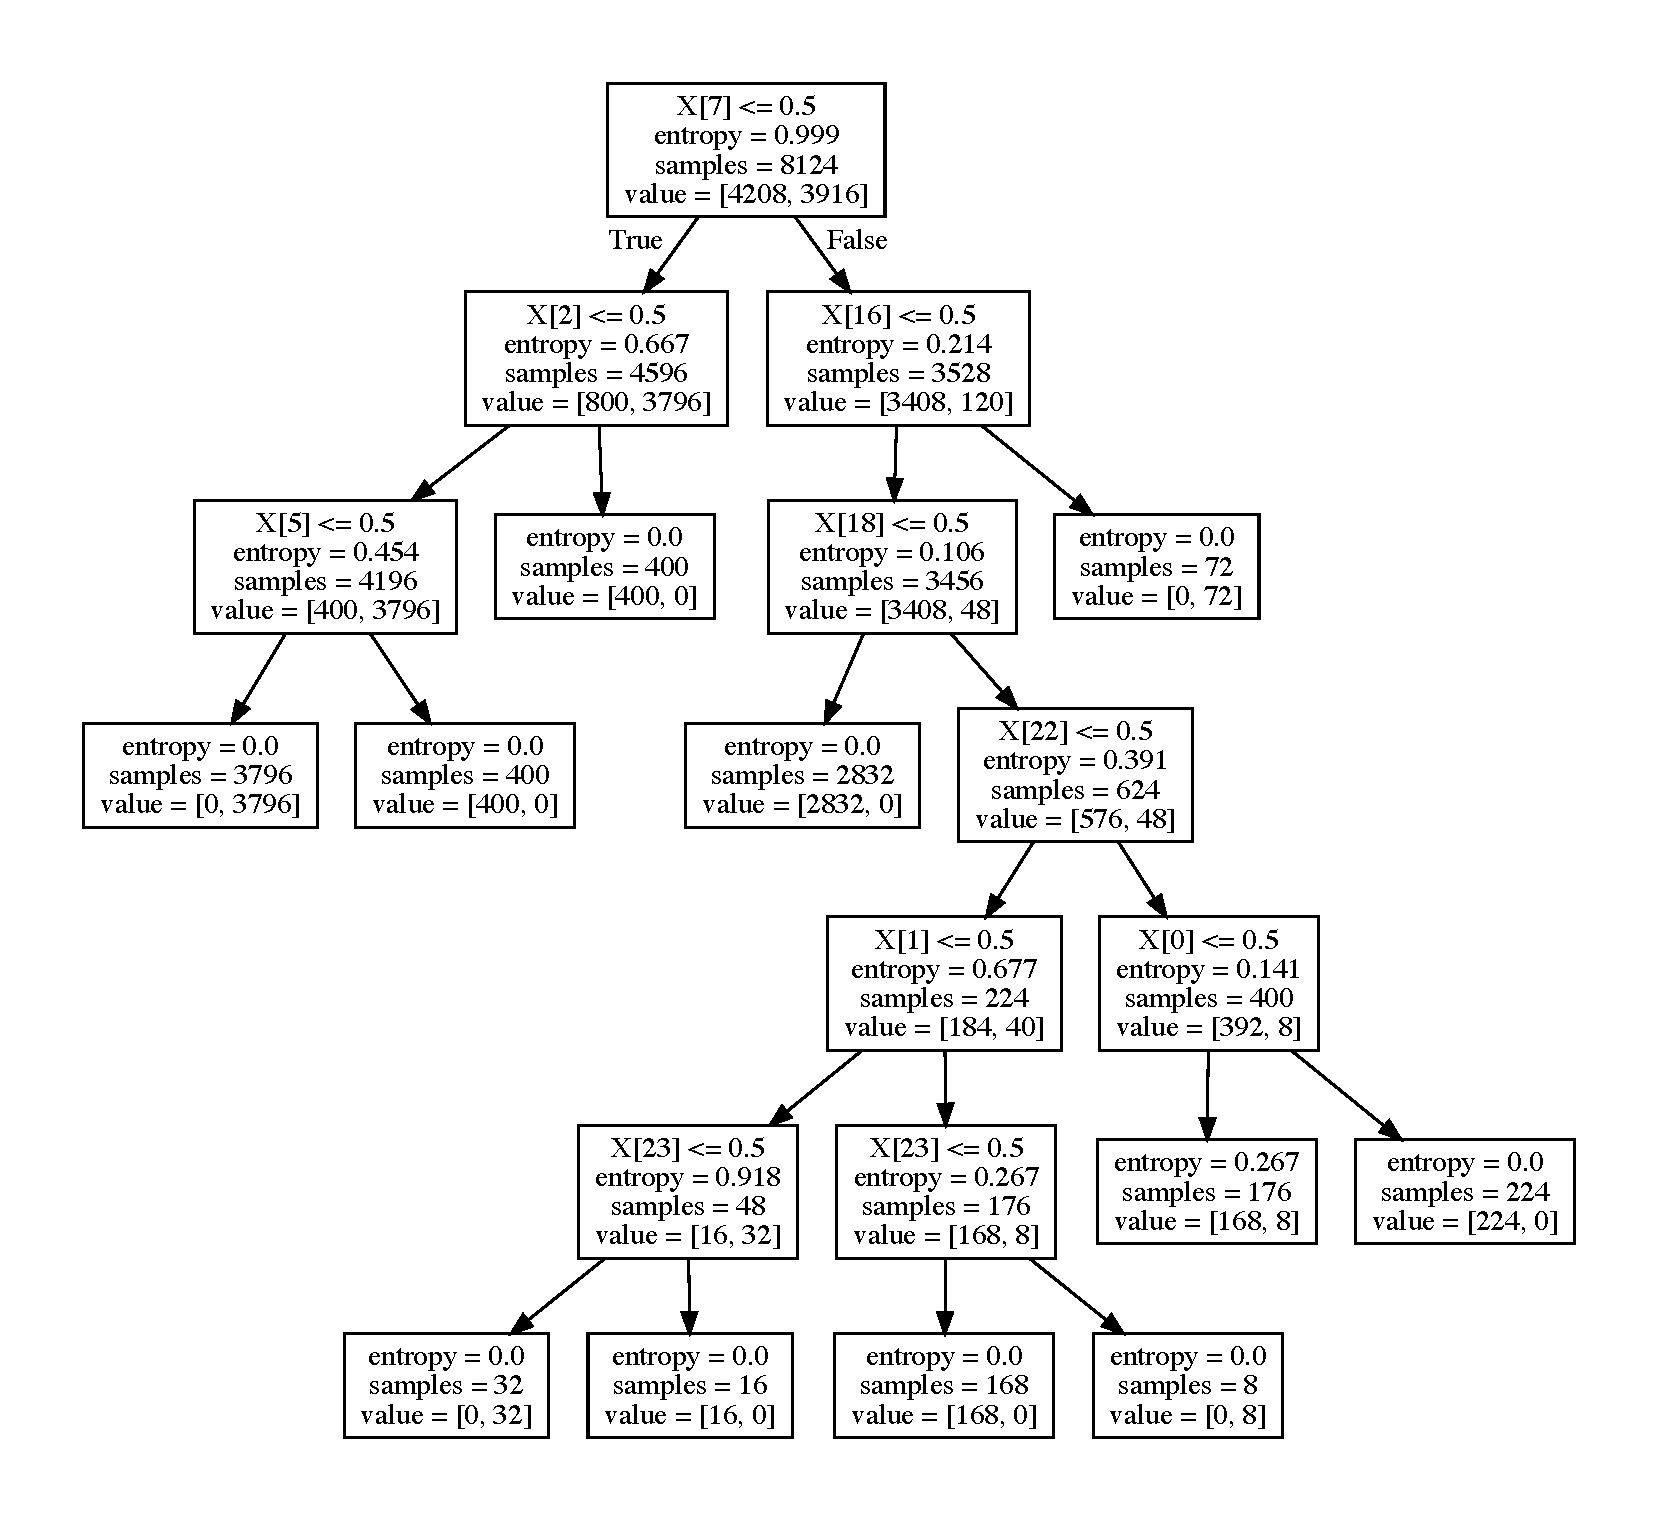
\includegraphics[scale=0.5]{tree4}
	\caption{GA process \& Decision Tree for 4 features}
	\label{fig-4}
\end{figure}

\begin{figure}[H]
	\centering
	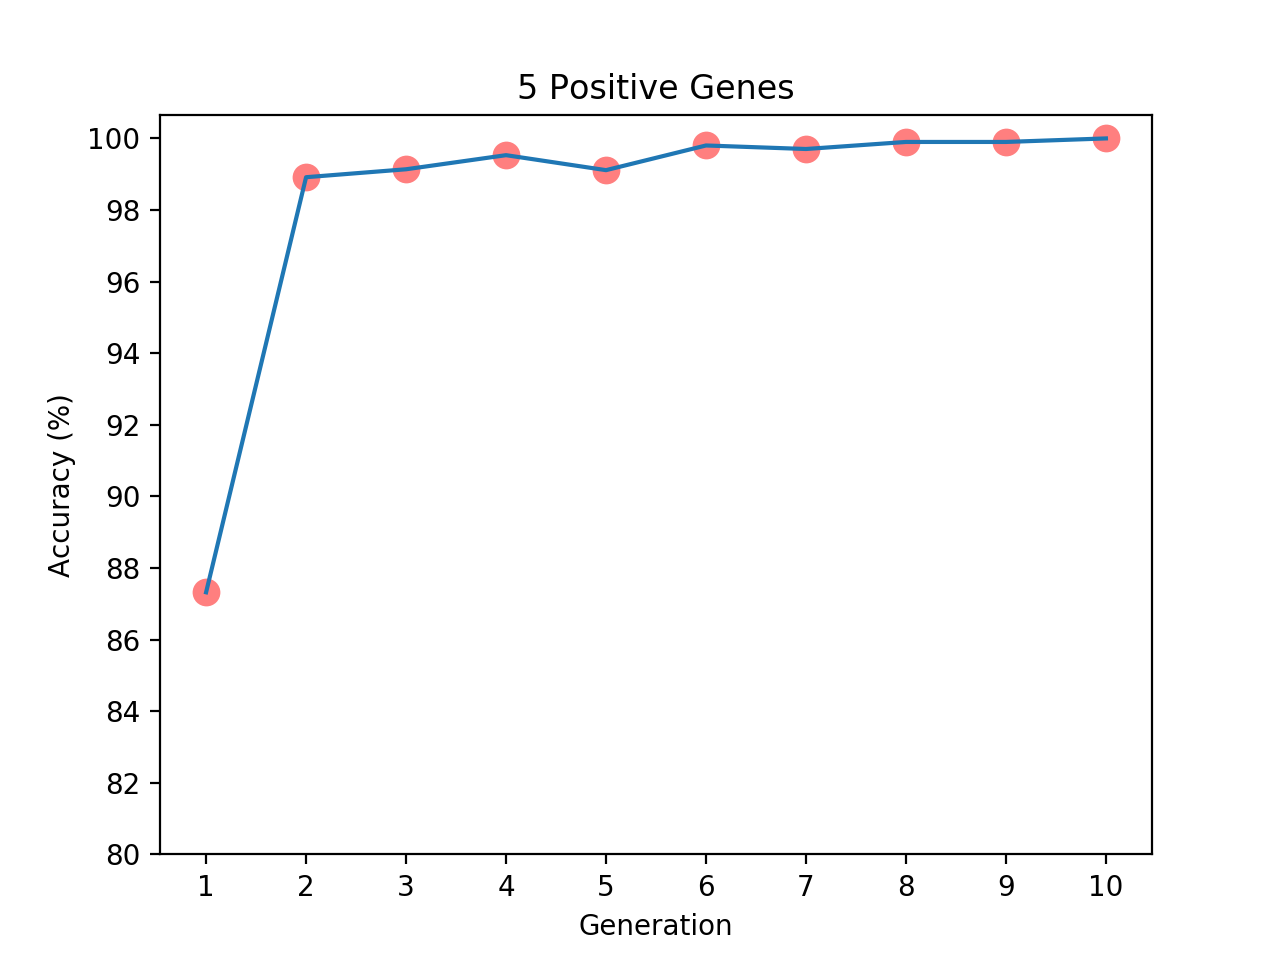
\includegraphics[scale=0.5]{GA5}
	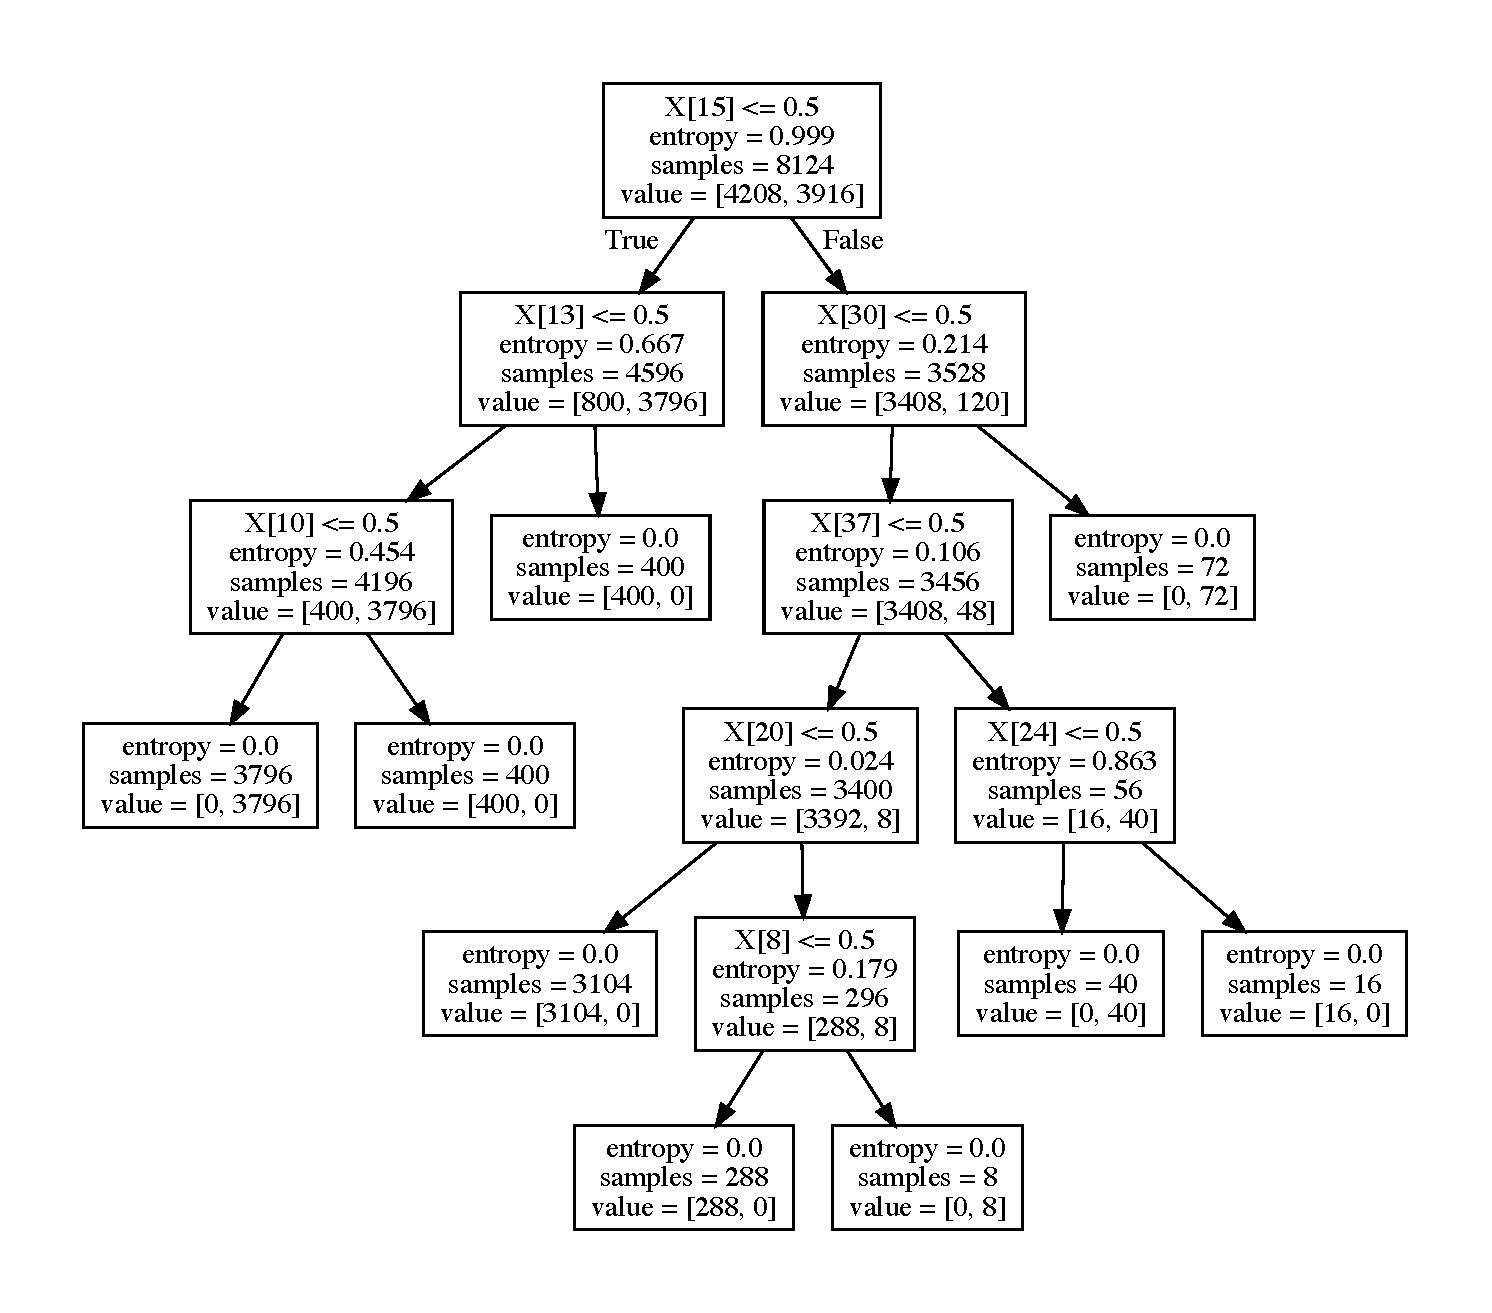
\includegraphics[scale=0.5]{tree5}
	\caption{GA process \& Decision Tree for 5 features}
	\label{fig-5}
\end{figure}

\section{Conclusion}
In this article, I aim at extracting crisp logical rules for mushroom edibility. Since all the variables are nominal (categorical) values, we need to quantize them first. My method is vectorized discretization. Then I have tried two different approaches to implement classification. The first method is to train back-propagation neural networks, with an auxiliary cost function term to force weight convergence. The second measure is Genetic Algorithm for feature selection plus Decision Tree.

In nature, logical rule extraction is essentially a task of feature selection. You select important features and then construct conditional logical rules. So GA is the better approach compared with neural networks intuitively. In reality, the method of BP neural networks relies largely on parameter adjustment; and may perform poorly and need improvements when things get complicated. GA + Decision Tree, by contrast, does not meet this trouble. Moreover, GA gives more illustrative information and supports manually changing a vital parameter---DNA\_POSITIVE (see Table~\ref{tab-GA}). However, the weak point is that GA runs slower than neural networks, probably because it needs to train plenty of Decision Trees.

\appendix
\section{GA Displays}
% DNA_POSITIVE = 3
\begin{verbatim}
----------DNA_POSITIVE = 3----------
Generation 1
Most fitted DNA: [0 0 0 0 0 1 0 0 0 0 0 0 0 0 0 0 0 0 1 0 1 0]
Accuracy = 89.36484490398819%
Generation 2
Most fitted DNA: [0 0 0 0 1 0 0 0 0 0 0 0 0 0 0 0 0 0 1 0 1 0]
Accuracy = 98.52289512555392%
... ...
... ...
Generation 10
Most fitted DNA: [0 0 0 0 1 0 0 0 0 0 0 0 1 0 0 0 0 0 0 1 0 0]
Accuracy = 99.70457902511079%
----------Final Decision Tree----------
Feature List:
['odor=a', 'odor=c', 'odor=f', 'odor=l', 'odor=m', 'odor=n', 'odor=p', 'odor=s', 'odor=y',
'spore-print-color=b', 'spore-print-color=h', 'spore-print-color=k', 'spore-print-color=n',
'spore-print-color=o', 'spore-print-color=r', 'spore-print-color=u', 'spore-print-color=w',
'spore-print-color=y', 'stalk-surface-below-ring=f', 'stalk-surface-below-ring=k',
'stalk-surface-below-ring=s', 'stalk-surface-below-ring=y']
DecisionTreeClassifier(class_weight=None, criterion='entropy', max_depth=8,
max_features=None, max_leaf_nodes=None,
min_impurity_decrease=0.0, min_impurity_split=None,
min_samples_leaf=1, min_samples_split=2,
min_weight_fraction_leaf=0.0, presort=False, random_state=None,
splitter='best')
Accuracy = 99.70457902511079%
\end{verbatim}

% DNA_POSITIVE = 4
\begin{verbatim}
----------DNA_POSITIVE = 4----------
Generation 1
Most fitted DNA: [0 1 1 0 0 0 0 0 0 0 0 0 0 0 0 0 0 0 1 1 0 0]
Accuracy = 92.86065977351059%
Generation 2
Most fitted DNA: [0 0 0 1 0 0 0 0 0 0 1 0 0 0 0 0 0 0 1 1 0 0]
Accuracy = 99.70457902511079%
Generation 3
Most fitted DNA: [0 0 0 1 0 0 0 0 0 0 1 0 0 0 0 0 0 0 0 1 0 1]
Accuracy = 100.0%
----------Final Decision Tree----------
Feature List:
['bruises?=f', 'bruises?=t', 'habitat=d', 'habitat=g', 'habitat=l', 'habitat=m', 'habitat=p',
'habitat=u', 'habitat=w', 'spore-print-color=b', 'spore-print-color=h', 'spore-print-color=k',
'spore-print-color=n', 'spore-print-color=o', 'spore-print-color=r', 'spore-print-color=u',
'spore-print-color=w', 'spore-print-color=y', 'stalk-root=?', 'stalk-root=b', 'stalk-root=c',
'stalk-root=e', 'stalk-root=r']
DecisionTreeClassifier(class_weight=None, criterion='entropy', max_depth=6,
max_features=None, max_leaf_nodes=None,
min_impurity_decrease=0.0, min_impurity_split=None,
min_samples_leaf=1, min_samples_split=2,
min_weight_fraction_leaf=0.0, presort=False, random_state=None,
splitter='best')
Accuracy = 100.0%
\end{verbatim}

% DNA_POSITIVE = 5
\begin{verbatim}
----------DNA_POSITIVE = 5----------
Generation 1
Most fitted DNA: [1 0 0 1 0 1 0 0 0 0 1 1 0 0 0 0 0 0 0 0 0 0]
Accuracy = 87.32151649433777%
Generation 2
Most fitted DNA: [0 0 0 1 1 0 0 0 0 0 1 1 0 0 0 0 0 1 0 0 0 0]
Accuracy = 98.91678975873953%
... ...
... ...
Generation 10
Most fitted DNA: [0 0 1 0 1 0 0 0 0 0 0 0 1 0 0 0 0 0 0 1 1 0]
Accuracy = 100.0%
----------Final Decision Tree----------
Feature List:
['cap-color=b', 'cap-color=c', 'cap-color=e', 'cap-color=g', 'cap-color=n', 'cap-color=p',
'cap-color=r', 'cap-color=u', 'cap-color=w', 'cap-color=y', 'odor=a', 'odor=c', 'odor=f',
'odor=l', 'odor=m', 'odor=n', 'odor=p', 'odor=s', 'odor=y', 'population=a', 'population=c',
'population=n', 'population=s', 'population=v', 'population=y', 'spore-print-color=b',
'spore-print-color=h', 'spore-print-color=k', 'spore-print-color=n', 'spore-print-color=o',
'spore-print-color=r', 'spore-print-color=u', 'spore-print-color=w', 'spore-print-color=y',
'stalk-surface-below-ring=f', 'stalk-surface-below-ring=k', 'stalk-surface-below-ring=s',
'stalk-surface-below-ring=y']
DecisionTreeClassifier(class_weight=None, criterion='entropy', max_depth=5,
max_features=None, max_leaf_nodes=None,
min_impurity_decrease=0.0, min_impurity_split=None,
min_samples_leaf=1, min_samples_split=2,
min_weight_fraction_leaf=0.0, presort=False, random_state=None,
splitter='best')
Accuracy = 100.0%
\end{verbatim}

%
% ---- Bibliography ----
%
% BibTeX users should specify bibliography style 'splncs04'.
% References will then be sorted and formatted in the correct style.
%
\bibliographystyle{splncs04}
\bibliography{references.bib}
%
% \begin{thebibliography}{4}
% \bibitem{ref_1}
% Milne, L. K., Gedeon, T. D., \& Skidmore, A. K. (1995). Classifying dry sclerophyll forest from augmented satellite data: comparing neural network, decision tree \& maximum likelihood. Training.

% \bibitem{ref_2}
% The Audubon Society Field Guide to North American Mushrooms (1981). G. H. Lincoff (Pres.), New York: Alfred A. Knopf

% \bibitem{ref_3}
% Schlimmer,J.S. (1987). Concept Acquisition Through Representational Adjustment (Technical Report 87-19).  Doctoral disseration, Department of Information and Computer Science, University of California, Irvine.

% \bibitem{ref_4}
% Adamczak, R., \& Grabczewski, K. (1996). Extraction of logical rules from training data using backpropagation networks.

% \end{thebibliography}
\end{document}
